We divide our object model into subvolumes, each consisting of a TSDF, 
colour volume and object probability volume, and contains a rigid body transform that specifies its pose relative to the global coordinate frame. At each new camera frame, we apply our segmentation model to the colour input image to construct an object probability map, and then accumulate the probabilities from this map into the object probability volume of the active subvolume (see Section~\ref{subsec:probfusion}). We also update the TSDF and colour volume of the active subvolume, and track against it using ICP. At the end of each frame, we run our novel online model correction algorithm (see Section~\ref{subsec:onlinemodelcorrection}), which infers the relative poses between the subvolumes to mitigate tracking drift. Once the reconstruction process is finished, we perform a CRF-based optimisation to refine the resulting object segmentation (see Section~\ref{subsec:shapeoptimisation}). Our approach is not tied to the use of any one probabilistic model, though in our experiments we use PwP (Pixel Wise Posteriors) \cite{Bibby2008}. An overview of our object reconstruction pipeline is shown in Figure~\ref{pipelineDiagram}.

\begin{figure*}[!t]
	\centering
	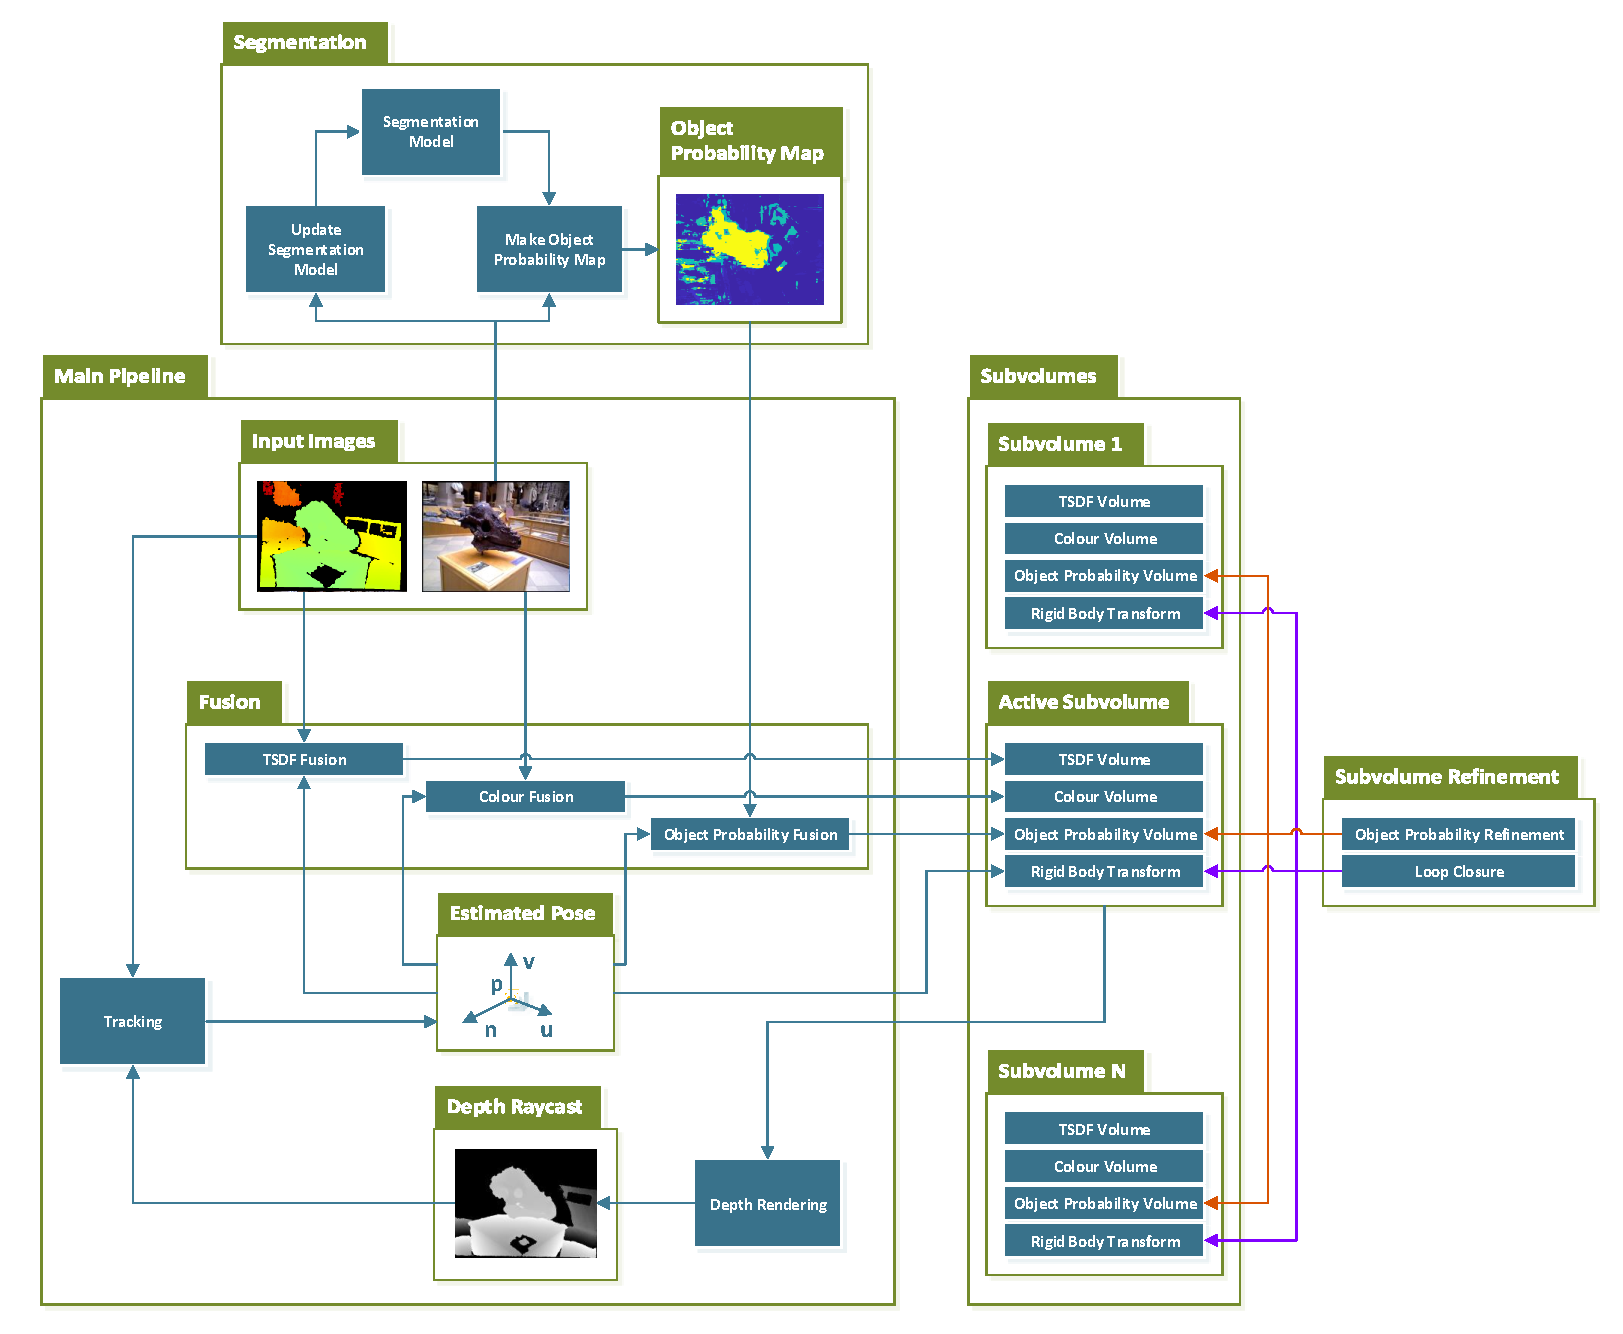
\includegraphics[width=0.7\linewidth]{pipeline.pdf}
	\vspace{-3mm}
	\caption{The pipeline of our object reconstruction approach.}
	\label{pipelineDiagram}
\end{figure*}

\subsection{Probabilistic Object Fusion Procedure}
\label{subsec:probfusion}

The surface map and camera pose are estimated using the standard pipeline of \cite{Newcombe2011,Prisacariu2014}. The surface is represented as the zero level set of a TSDF discretised over voxels, with online weighted-mean fusion of new observations. Pose estimation via ICP is run quasi-simultaneously against the evolving map. Here, inspired by \cite{Kolev2006}, we augment this procedure by estimating the posterior probability, per map voxel, of belonging to the object. This volume of posterior probabilities is updated on each frame, parallel to the fusion process in the mapping and pose estimation subsystems. The representation of the reconstructed object comprises multiple `subvolumes', each pertaining to some patch on the object surface. New subvolumes are started when sufficiently many new voxels have been allocated and have had data integrated. By ensuring overlap between subvolumes, transformations between them can be found and pose inconsistencies addressed, online. Empirically, we define the threshold for starting a new subvolume to be when $50\%$ of the voxels fused in to the current volume are newly observed points.

At each frame, the object probabilities for the visible voxels in the active submap are updated via an appearance-derived probability map for that frame. Under the assumption of conditional independence between frames (for sake of tractability), the posterior probability of a given voxel $\psi \in \Psi$ belonging to the object has the following form (noting that $\Phi \subset \Psi$):
\begin{equation}
\label{eq:membership}
\begin{split}
P(\psi \in \Phi | \Omega, p) = \prod_{t=0}^{\infty} P(\psi_{t} \in \Phi | \Omega_{t}, p_{t})
\end{split}
\end{equation}
where $\Psi$ is the volume of voxels for which measurements are accumulated, $\Phi$ 
is the volume of voxels pertaining to the object, $\Omega_{t}$ is the current image observation at time $t$ and $p_{t}$ is the currently tracked pose at time $t$.
This encodes the probability of a voxel belonging to the object as the product of instantaneous appearance-derived pixel-wise conditionals.
%(In the above, $\Phi$ is a discretisation of the continuous $\Phi$ in the probabilistic formulation that follows.)

\subsection{Probabilistic Formulation of Object Reconstruction}
Central to the proposed system is a volume of posterior probabilities pertaining to a voxel wise membership of either the 
object set or the non object set. This allows formulation of the full joint distribution over the object as the Probabilistic 
Graphical Model of Figure \ref{fig:pgm}(left).

\begin{figure}[!t]
	\centering
	\begin{tabular}{cc}
		%\fbox{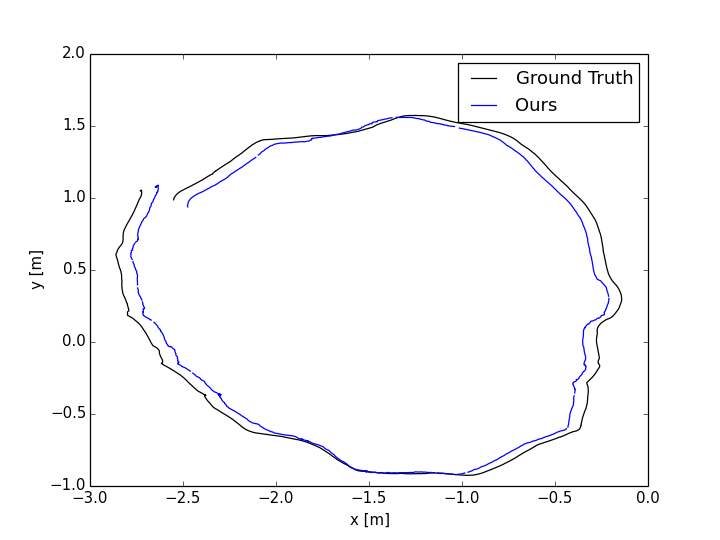
\includegraphics[width=0.2\textwidth]{results/rgbd_dataset_freiburg3_cabinet.png}} & %\fbox{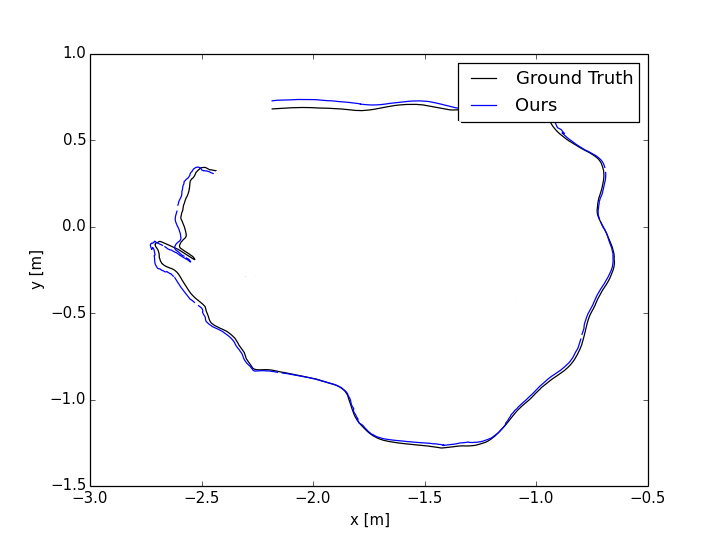
\includegraphics[width=0.2\textwidth]{results/rgbd_dataset_freiburg3_teddy.png}}
		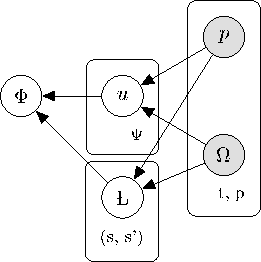
\includegraphics[height=3cm]{graphical_models/pgm1.pdf}&
		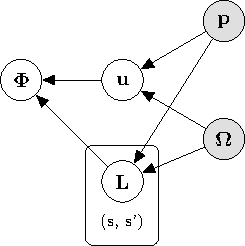
\includegraphics[height=3cm]{graphical_models/pgm2.pdf}
		\vspace{-3mm}
	\end{tabular}
	\caption{An initial probabilistic formulation of the object reconstruction pipeline (left) and a simpler formulation based on various independence assumptions (right).}
	\label{fig:pgm}
\end{figure}

Where $\Phi$ is the shape to be reconstructed (represented as a subset of voxels for which surface data has been integrated), $u$ is the appearance model volume, $L$ is the 
set of consistency constraints for each adjacent sub volume pair in the form of rigid transformations, $\Omega$ is the set of 
RGBD image pixels and $p$ the set of poses over time.

This gives rise to the following factorisation of the distribution given in Figure \ref{fig:pgm}(left)
\begin{equation}
\begin{split}
P(\Phi, \Omega, p, u, L) = 
\prod_{\psi \in \Psi}\prod_{s, s' \in \mathcal{S}}P(\Phi|u_{\psi}, L_{s, s'}) 
\prod_{t=0}^{\infty}\prod_{p \in \mathcal{P}}\\
P(u_{v}|\Omega_{p, t}, p_{t})
P(L_{s, s'}|\Omega_{p, t}, p_{t})
P(L_{s, s'})P(p_{t})P(\Omega_{p, t})
\end{split}
\end{equation}
where $\Psi$ is the set of voxels across all sub volumes, $\mathcal{P}$ is the set of RGBD pixels for a given 
frame and $\mathcal{S}$ is the set of sub volumes. Where the notation $s, s' \in \mathcal{S}$ refers to pairs of overlapping subvolumes.

However, if pixel wise independence is assumed in the RGBD observations and temporal independence in 
the poses, the plate containing $\Omega$ and $p$ can be removed as in Figure \ref{fig:pgm}(right).
\begin{equation}
\begin{split}
P(\Phi, \Omega, p, u, L) = 
\prod_{v \in \mathcal{V}}P(\Phi|u_{v})
\prod_{s, s' \in \mathcal{S}}P(u_{v}|\Omega, p, L_{s, s'}) \\
P(L_{s, s'}|\Omega, p) P(L_{s, s'})P(p)P(\Omega)
\end{split}
\end{equation}
In practice this temporal independence assumption causes no issues. Furthermore, if voxel wise independence is assumed, the plate over voxels can be removed. Finally, assuming $P(p)$ and 
$P(\Omega)$ are uniform distributions, then we have the simpler distribution given by Figure \ref{fig:pgm}(right).

\iffalse
\begin{figure}[!t]
	\centering
	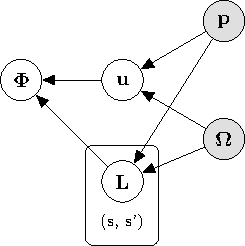
\includegraphics{graphical_models/pgm2.pdf}
	\caption{Simplified probabilistic formulation of the object reconstruction pipeline.}
	\label{pgm2}
\end{figure}
\fi

This simpler distribution can be factorised as follows
\begin{equation}
\begin{split}
P(\Phi, \Omega, p, u, L) = 
\prod_{s, s' \in \mathcal{S}} P(\Phi|u, L_{s, s'}) \\
P(u|\Omega, p)
P(L_{s, s'}|\Omega, p)
P(L_{s, s'})
\end{split}
\end{equation}

The above formalisms describe a probabilistic framework in which online corrections can be made to the reconstructed model to counteract 
errors incurred by pose tracking inconsistencies. As with scene based dense SLAM systems \cite{Newcombe2011, Prisacariu2014, Niessner2013}, 
our system follows a pipeline that consists of a tracking stage and an integration stage. However, our formulation of this pipeline 
consists of an additional, novel estimation module that relies on the use of a subvolume representation to correct tracking errors by applying 
transformations to the subsegments to align them when there are intra subsegment tracking inconsistencies. 
As inference on the joint distribution of our model is intractable, conditional independence assumptions are made that do not appear 
to cause any functional issues.

\subsection{Online Model Correction}
\label{subsec:onlinemodelcorrection}

The tracking consistency constraint denoted by the variable $L$ in the graphical models given by Figure \ref{fig:pgm} can 
be enforced in terms of minimising the disparity between adjacent subvolumes, such that the poses tracked in each subvolume are consistent.  
%The approach proposed in this work differs from \cite{Kahler2016} in that the optimisation is integrated in to the probabilistic formulation previously outlined. 
Given instantaneously inferred transforms between subvolumes obtained from tracking results, 
the objective is to infer a robust, consistent deformation transformation for the subvolume pair.
As such, for each pair of visible subvolumes $s, s'$, the following posterior must be maximised:
\begin{equation}
\begin{split}
%Bayes rule + chain rule for P(omega, p)
P(\Omega, p | L_{s, s'}) = \frac{P(L_{s, s'} | \Omega, p) P(\Omega | p)P(p)}
{P(L_{s, s'})}
\end{split}
\end{equation}
The intuition behind the above equation is that the deformation $L_{s, s'}$ applied to the object subvolume $\Phi_{s}$ should 
increase the probability of observing the current pose $p$ given the current RGBD frame $\Omega$ by reducing the 
variance of the pose estimation result. As such, global tracking variance is reduced by enforcing local consistency, improving the quality 
of the reconstruction.

It should be noted that in our implementation the $P(\Omega | p)$ term is assumed to be uniform in the case of an 
RGBD sensor being used, however for applications such as monocular SLAM this term may be replaced with a noise model when there is 
significant uncertainty about the given depth map at each frame.
The following proportionality to the distribution over deformations is made for two overlapping object subsegments $\Phi_{s}, \Phi{s'} \in \Phi$, noting again that 
$\Phi \subset \Psi$. $X$ is the set of valid voxel locations in $\Phi_{s}$ for which the currently accumulated appearance posterior is greater for foreground:
\begin{equation}
\begin{split}
P(L_{s, s'} | \Omega, p) \propto P(\Phi_{s}(X)) | \Phi_{s'}(\Lambda(X))P(L_{s, s'})
\end{split}
\end{equation}
Where the prior distribution over transformations $P(L_{s, s'})$ corresponds to the Gaussian Conjugate Prior $\mathcal{N}(L_{s, s'} | \mathbf{0}, \mathbf{\lambda}^{-1})$.
The log posterior of the above expression takes the following form:
\begin{equation}
\label{eq:logPosterior}
\begin{split}
\ln P(\Phi_{s}(x) | \Phi_{s'}(\Lambda(x)))P(L_{s, s'}) = m\ln\frac{1}{\sqrt{2\pi}\sigma} -\frac{1}{2\sigma^2} \\ 
\sum_{\psi \in \Phi_{s}} \Bigg [ \bigg( \Phi_{s}(x_{\psi}) - \Phi_{s'}(\Lambda(x_{\psi})) \bigg)^2  - \lambda \lVert \mathbf{\mathbf{x}} \rVert_{2} \Bigg ]
\end{split}
\end{equation}
Where $\Phi_{s}(.)$ is a scalar valued SDF (Signed Distance Function) for the subsegment $s$, a discretised field of $\Phi_{s}$ (where $\Phi_{s} \subset \Phi$), as previously described. $x$ is a point represented by a 3-vector and $\Lambda(.)$ is a transformation function taking the following form:
\begin{equation}
\begin{split}
\Lambda(x) = R(\rho_{1}, \rho_{2}, \rho_{3})x + t
\end{split}
\end{equation}
Where $R(.)$ is a rotation matrix from the Special Orthogonal group $\mathbbm{SO}(3)$ parameterised by the three 
Rodrigues Parameters \cite{Shuster1993} $\rho_{1}$, $\rho_{2}$ and $\rho_{3}$. The $\mathbf{x}$ in the log posterior refers to the vector $\mathbf{x} = [t_{1}, t_{2}, t_{3}, \rho_{1}, \rho_{2}, \rho_{3}]$, 
the translational and rotational parameters. Finally, $m$ is the number of voxel locations for which a valid SDF value has been found for both subsegments. In our experiments, $\sigma = 2$.\\
Note that the logarithmic form of the posterior is suitable to non-linear least squares optimisation. Gradient-based maximisation of the above posterior to yield an optimal deformation is a highly non-linear optimisation problem. As such, it is suited to second-order gradient-based optimisation. To perform MAP (Maximum A Posteriori) over this posterior using 
an optimisation routine such as Levenberg-Marquardt, the following gradients must be computed for the rotational component of the 
deformation:
\begin{equation}
\begin{split}
\frac{\partial E}{\partial \rho_{n}} = \frac{\partial E}{\partial \Psi} \frac{\partial \Psi}{\partial \Lambda} \frac{\partial \Lambda}{\partial \rho_{n}} \text{for } n \in \{1,2,3\}
\end{split}
\end{equation}
Similarly for the translational component:
\begin{equation}
\begin{split}
\frac{\partial E}{\partial t_{d}} = \frac{\partial E}{\partial \Psi} \frac{\partial \Psi}{\partial \Lambda} \frac{\partial \Lambda}{\partial t_{d}} \text{for } d \in  \{x,y,z\}
\end{split}
\end{equation}
where the gradient $\frac{\partial \Psi}{\partial \Lambda}$ is found via central finite differencing.
For notational convenience we define $E \equiv \ln P(\Phi_{s}(x) | \Phi_{s'}(\Lambda(x)))P(L_{s, s'})$, see Equation \ref{eq:logPosterior}

\subsection{Implicit Surface Deformations}
%In the previous section, a model and estimation procedure was presented to find optimal transformations between the aforementioned subvolumes.
The overall object surface $\Phi$ is implicitly deformed by a blending function $\zeta(\Phi)$ over each of the subvolumes for which surface data has been integrated.
As such the surface $\Phi$ is given by the following:
\begin{equation}
\begin{split}
\Phi(\mathbf{x}) = \sum_{\chi \in X} \zeta(\Psi_{\chi}(\mathbf{x}))
\end{split}
\end{equation}
where $X$ is the set of subvolumes contributing to the surface $\Psi$. As such, the previously described transformation estimation process that deforms each of the subvolumes, implicitly optimises 
for the true surface as depicted in Figure \ref{fig:deformationDiagram}.
\begin{figure}[!t]
	\centering
	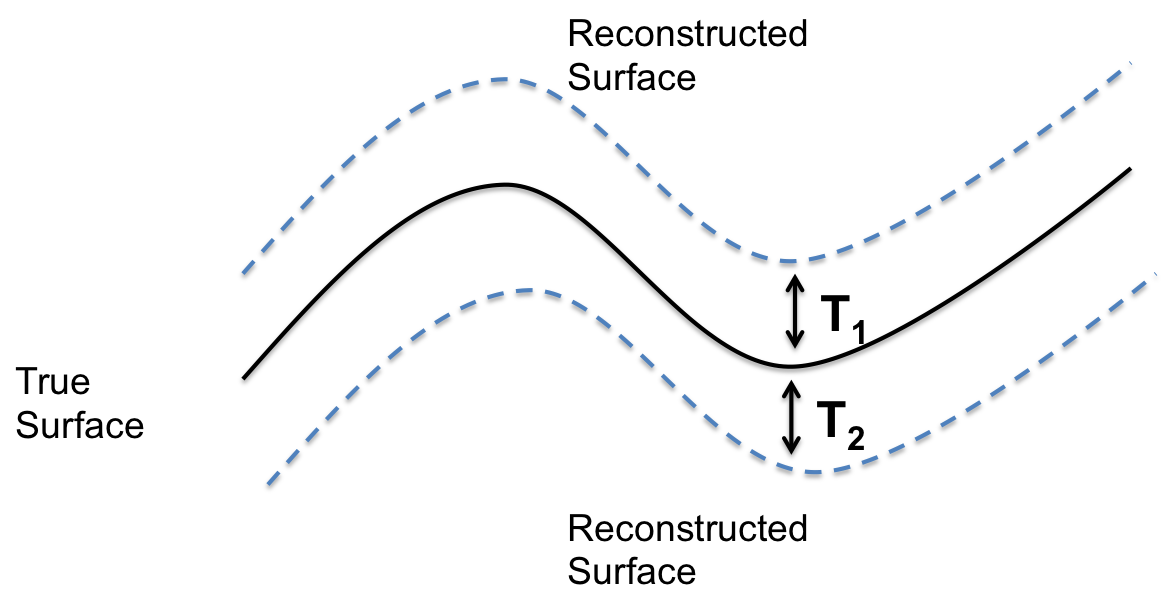
\includegraphics[scale=0.25]{deformation.png}
	\vspace{-3mm}
	\caption{Measured surfaces from different subvolumes being deformed to the true surface.}
	\label{fig:deformationDiagram}
\end{figure}
In our experiments $\zeta (.)$ is defined as follows
\begin{equation}
\begin{split}
\zeta(\psi_{\chi}) = 
\begin{cases}
\psi_{\chi} & \text{if $P(\psi \in \mathbf{\Phi} | \Omega, p) > P(\psi \notin \mathbf{\Phi} | \Omega, p)$} \\
0 & \text{if $P(\psi \in \mathbf{\Phi} | \Omega, p) < P(\psi \notin \mathbf{\Phi} | \Omega, p)$}
\end{cases}
\end{split}
\end{equation}
At this point the reader is referred back to Equation \ref{eq:membership}.

\subsection{Volumetric Object Segmentation}
\label{subsec:shapeoptimisation}
The final stage in the proposed object reconstruction pipeline is the segmentation of the object voxels from those that have had measurements fused 
from the background. This segmentation is formulated within a CRF framework, where each node in the CRF represents a set of neighbouring voxels in space, 
with connections being made between adjacent neighbourhoods. The process of segmentation can be posed as an energy minimisation problem over a cut in downsampled voxel space, 
such that a segmentation in 3D is obtained. The following energy function consists of the unary posterior probabilities over appearance accumulated during the fusion 
process for a region in space and an additional pairwise smoothing term representing the physical appearance similarity of the object region represented by the voxel 
neighbourhoods $\gamma$ and $\gamma^{'}$:
\begin{equation}
\begin{split}
E_{n} = \prod_{t=0}^{\infty} \prod_{\psi \in \Phi_{n}} P(\psi \in \Psi | \Omega_{t}, p_{t}) + P(\mathbb{E}[c]_{\gamma} | \mathbb{E}[c]_{\gamma^{'}})
\end{split}
\end{equation}
where $c$ represents the set of colour measurements fused in to the voxels within a given neighbourhood, for all $N$ subvolumes and $\mathbb{E}$ is the standard Expectation operator.
The aforementioned cut in voxel space is achieved by an optimisation of the above equation within the Max-Flow framework \cite{BoykovKolmogorov}. 
%At this point, it should be reiterated that the unary term in the above equation is the accumulated(during reconstruction) foreground vs background probability.

\subsection{Explicit Loop Closure Detection}
In addition to our online model correction algorithm to counteract tracking drift, we also detect loop closure events such that re-localisation can occur and 
the tracked pose be adjusted accordingly. Following the approaches of \cite{Glocker15,Kahler2016} we utilise a keyframe-based loop closure detection system. For a 
given depth image, its corresponding keyframe is a subsampled and Gaussian filtered version of the depth image which is then encoded in a Fern Conservatory. 
Similarity/dissimilarity scores between Ferns are then computed and used to either detect a loop closure event for high scoring matches with existing keyframes, 
or to spawn a new keyframe if dissimilarity is sufficiently high w.r.t.\ the last keyframe.

\subsection{Surface Fusion Procedure}
\paragraph{Volumetric Representation}
The system we present follows the KinectFusion \cite{Newcombe2011} pipeline for the integration of surface information. In such a 
formulation the scene or object is represented as the zero level of a level set embedding \cite{Curless1996}, where the level set is a field of distances 
to the surface. The surface itself is given by
\begin{equation}
	\begin{split}
		S = \left\{\psi | \mathcal{D}(\psi) = 0\right\}
	\end{split}
\end{equation}
where $S$ is the set of surface voxels, $\psi$ is a voxel in the SDF(Signed Distance Function) volume and $\mathcal{D}(.)$ is the SDF value. 
The SDF volume is truncated to yield a TSDF with truncation region $\mu$.

\paragraph{Pose Estimation}
The pose estimation method used in this work is the ICP algorithm \cite{Besl1992}. The estimation of 
the camera or object 6-DoF(Degree of Freedom) pose is formulated as a minimisation problem of the form:
\begin{equation}
	\begin{split}
		\arg \min_{R, t} E = \sum_{\omega \in \Omega_{d}} \bigg( \big( R\omega + t - \mathcal{V}(\bar{\omega}) \big) \cdot \mathcal{N}(\bar{\omega}) \bigg)^{2}
	\end{split}
\end{equation}
where $\Omega_{d}$ is a depth image, $\omega$ is a 3D point extracted from the depth image, $R$ is an  $\mathbbm{SO}(3)$ 
rotation matrix, $t$ is a translation vector, $\mathcal{V}$ is a rendered depth map from the SDF model, $\mathcal{N}$ is a rendered 
normal map from the SDF model and $\bar{\omega}$ is the point $\omega$ projected from the coordinate frame of $\mathcal{V}$ and 
$\mathcal{N}$ to the image plane. At this point it should be highlighted that the tracking algorithm used is separate from the contributions in this paper and 
as such can be substituted for any suitable pose estimation algorithm.

\paragraph{Surface Integration}
We utilise a weighted mean to fuse new depth measurements in to the TSDF model, as such, for a new depth measurement $\eta$ projected to by voxel $\psi$, 
the following update to the TSDF volume $\mathcal{D}$ is made
\begin{equation}
	\begin{split}
		\mathcal{D}'(\psi) \leftarrow \frac{w(\psi)\mathcal{D}(\psi) + \min(1, \eta/\mu)}{w(\psi) + 1}
	\end{split}
\end{equation}
where $w(.)$ is a weighting function and $\mu$ is the aforementioned TSDF truncation region.